%!TEX root = ../thesis.tex
\chapter{Experiments}
In this chapter, both proposed heterogeneous pc-stable algorithm approaches are evaluated. Furthermore, two different systems are used for the evaluation to elaborate the hardware dependency of the heterogeneous version.

\section{Setup}
The dataset the experiments use for computation is based on the dataset used in the experiments of Perscheid et al. \cite{perscheidIntegrativeGeneSelection2018}. The dataset is taken from The Cancer Genome Atlas (TCGA) \cite{weinsteinCancerGenomeAtlas2013}. Genes with more than 30\% missing values are filtered out. The remaining data is normalized and log-transformed. The original dataset consists of 55 573 variables. While the run-time of the PC stable algorithm grows exponentially with the variable count, subsets of the dataset are used for evaluation. The subset sizes chosen for the evaluation are 1000 variables, 10 000 variables, and 45 000 variables. The 1000 variables dataset is used to represent small datasets and will be called TCGA-1000. The 10 000 variables dataset is a large dataset that does not fill the memory of the system's GPU. The 45 000 variables dataset is therefore used to show the effects of GPU memory overflow on the algorithms execution time in this evaluation.

\begin{figure}[h]
  \caption{System 1 Architektur - Delos}
  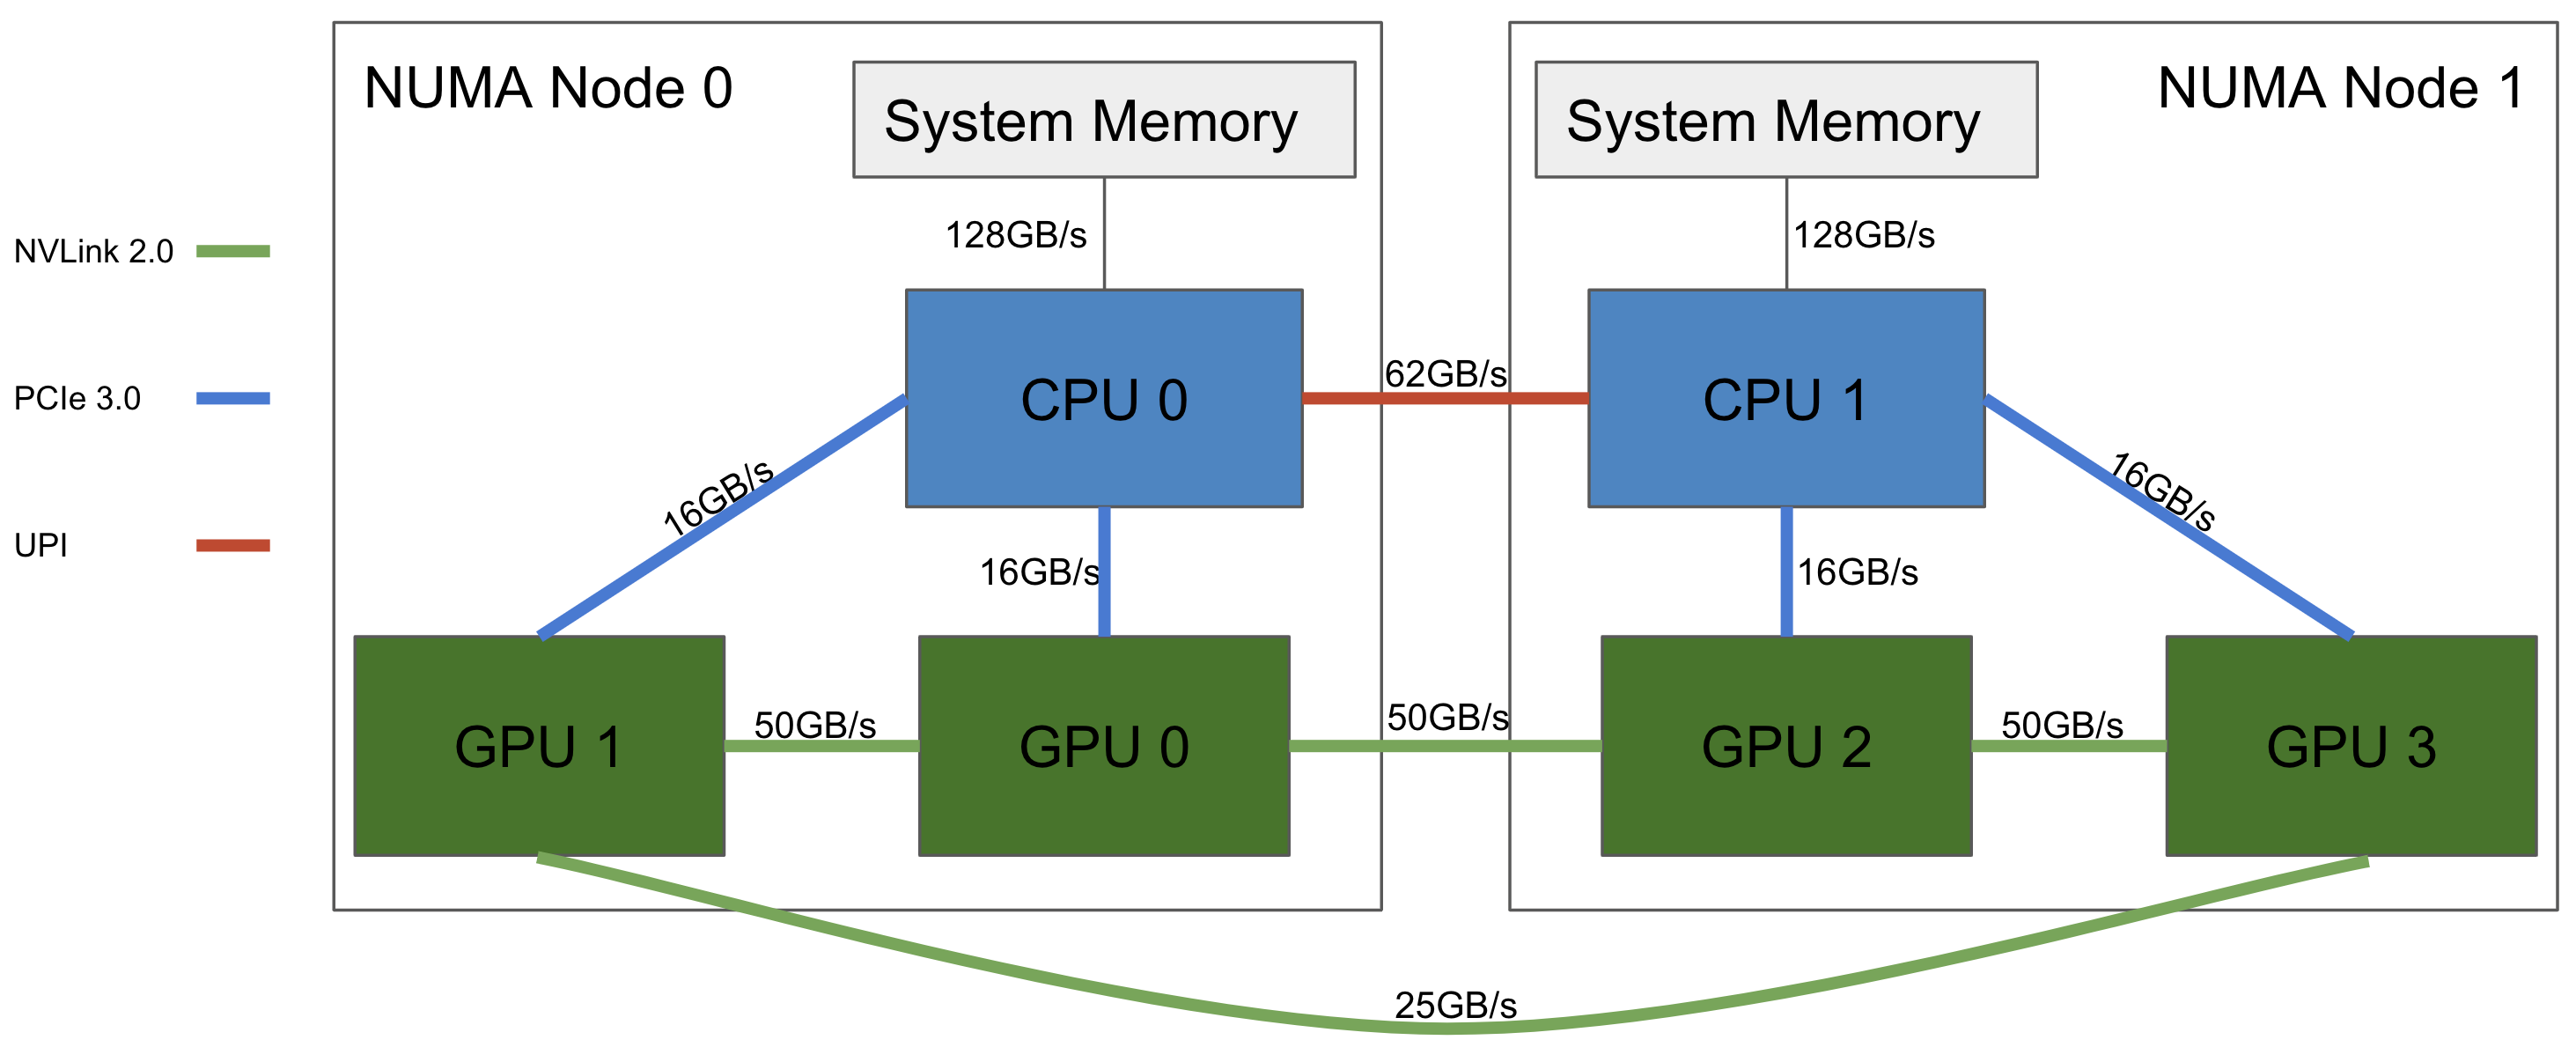
\includegraphics[width=\textwidth]{figures/delos_system_arch.png}
  \centering
  \label{fig:delos_arch}
\end{figure}

Two different systems are used for the evaluation. One system, which will be called Delos \ref{fig:delos_arch} in the following, consists of 4 Nvidia Tesla V100 GPUs with each 32GB of SXM2 memory and 2 Intel Xeon Gold 6148 CPUs with each 755GB of DDR4 memory. The Tesla V100 GPU clock rate is 1,53 GHz. It contains 80 Streaming Multiprocessors which each can execute a maximum of 2048 threads concurrently \cite{NVIDIATESLAV1002017}. The Intel Xeon Gold 6148 has 20 cores with a clock rate maximum of 3,70 GHz. Each core has two so-called hyper threads so that the CPU can execute 40 threads concurrently.

The second system, which will be called AC922 in the following, is a high-performance computing system developed in collaboration with IBM and Nvidia \cite{caldeiraIBMPowerSystem}. It incorporates the same GPUs as the Delos system (4xNvidia Tesla V100) and two IBM Power9 processors. Each Power9 processor has 16 cores with a clock rate maximum of 4 GHz, which, by using SMT4 multithreading, can execute 64 threads concurrently. 256GB DDR4 RAM is connected to each CPU.

Through the collaboration of IBM and Nvidia, the interconnect between a CPU and GPU in this system is NVLINK \cite{NVLink2021, zargesEvaluationOnNodeGPU} with a bandwidth of 150GB/s in contrast to the Delos PCIe 3.0 16GB/s interconnect. NVLINK is also faster latency wise \cite{liEvaluatingModernGPU2020}. This allows for evaluating bottlenecks regarding interconnect speed in this heterogeneous computation scenario.
Furthermore the collaboration brings other features which a heterogeneous computing application can benefit from, such as Adress Translation Services \cite{ibmpower9nputeamFunctionalityPerformanceNVLink2018} unifying the GPU and CPU page table, native atomics support for system wide accessible memory and direct GPU memory access by the CPU \cite{UNIFIEDMEMORYP9}.

The following experiments only use one GPU for execution, even if the proposed algorithm can be executed on multiple GPUs at once. Therefore parameters, such as GPU-GPU memory handling and interconnect technology, do not influence the CPU-GPU computation results. Some benchmarks are pinned to the NUMA node closest to the executing GPU to limit interconnect effects not related to the direct CPU-GPU connection. Both systems' CPUs are each directly connected to two GPUs, whichs means using only half the cores and memory while NUMA pinned. The largest dataset being used with the size of 36GB$\sim$ will not be the limiting factor for the CPU's associated memory of 755GB on Delos and 256GB on AC922. On the other hand, 36GB$\sim$ of data will fill the GPU's memory of 32GB which is intentional behavior as said above.

\section{Benchmarks}

At first basic experiments on the delos system are done, that refer to the 
% TODO add structured listing of experiments done

\subsection{Benchmarks Delos}
The first experiments
\begin{table}[h!]
  \centering
  \begin{tabular}{||c c c c||} 
   \hline
   Col1 & Col2 & Col2 & Col3 \\ [0.5ex] 
   \hline\hline
   1 & 6 & 87837 & 787 \\ 
   2 & 7 & 78 & 5415 \\
   3 & 545 & 778 & 7507 \\
   4 & 545 & 18744 & 7560 \\
   5 & 88 & 788 & 6344 \\ [1ex] 
   \hline
  \end{tabular}
  \caption{Table to test captions and labels}
  \label{table:1}
\end{table}

\subsection{Benchmarks AC922}


% - Explain dataset used for testing (TCGA)
%   - Variable size
%   - how sampled
%   - paper (perscheid etc)
% - Show delos as a testing machine
%   - Intel Xeon 
%   - Nvidia  V100
%   - specs
%   - numa nodes
% - Show AC922
%   - Explain why power9 + V100 special
%   - ATS: Malloc is enough
%   - Faster interconnect NVLINK
%     - Comparison between interconnects
%   - Other pros : atomics etc
%   - Explain why this should affect my performance
%   - Compare Power9 to Intel Xeon
% - Show iteration measurements per level
%   - show how many tests and iterations have to be done

% - Measurements of GPU only Code

% - Measurements of Pre-balanced
%   - With, without migrating edges
%   - Different thresholds
%   - Different Dataset sizes
%   - Different omp scheduling methods
%   - Pinning on NUMA nodes
%   - Delos vs AC922
% - Measurements of Workstealing
%   - With, without migrating edges
%   - Different Dataset sizes
%   - Pinning on NUMA nodes
%   - Delos vs AC922

% - Measurements with different Datasets
%   - Iterations
%   - Workstealing Numa 0
%   - Prebalanced
%   - GPU only
